%%% -*-LaTeX-*-

\chapter{Introduction}
\label{ch:introduction}
From the cosmic scale of astronomy to the atomic scale of chemistry, and from speculative economics to precision engineering, experts in a variety of fields are interested in gathering data in order to better understand the functional relationships between target quantities of interest and their presumed drivers.
%
For instance, what chemical or structural characteristics of a nuclear fuel optimize its safety and efficiency and to what degree and under what conditions?
%
Or to take an example from a different field, what socio-economic factors play the largest role in determining quality of life?
%
For abstract notions such as ``safety'' and ``quality of life'' that can be encoded numerically and measured or simulated, the scientific community has been designing analysis tasks capable of answering these types of questions.
%
Such tasks include identifying paramaters of interest from a field of candidates, efficient collection of data relating the candidate parameters to the outputs, identifying and summarizing trends in the functional relationship of the input space and output space, and building efficient and reliable predictive models.

However, many new and yet unexplored ideas lie at the intersection of fields of study such as statistics, geometry, and visualization.
%
As such, it is important to apply validated ideas from these disparate fields in order to augment and enhance solutions to problems occuring in other areas.
%
By combining complementary techniques, we can gain new understanding about our observed data and even inform the data gathering process.
%
One such field of recent interest is topological data analysis (TDA).
%
TDA is a growing field arising from the combination of computational geometry, topology, set theory, and visualization.

In this work, I investigate the efficacy of topological data analysis (TDA) techniques to problems arising in the realm of uncertainty quantification and risk monitoring.
%
In particular, I place a special emphasis on applications relevant to nuclear safety, such as adaptive sampling, sensitivity analysis, regression, limit surface extraction, and visualization of risk-informed datasets.
%
\textbf{By approximating topological constructs from potentially sparsely
sampled data, we are able to extract and analyze the structure of scientific simulation data stemming from low (one to three) to moderate (on the order of tens) dimensional input spaces to provide actionable insight for domain
scientists.}

This introductory chapter will qualify what kind of data this work applies to and will introduce the specific problem domain areas.
%
Chapter~\ref{ch:definitions} will normalize our language by synthesizing the relevant information from several fields including: data analysis, set theory, algebra, topology, and graph theory.
%
Chapter~\ref{ch:related} frames the contributions of this work in the context of related research and the current state of the art.
%
Chapter~\ref{ch:theory} addresses the theoretical aspects of the work involved by giving a thorough background on the topological constructs used throughout this body of research.
%
Chapters~\ref{ch:adaptiveSampling} and~\ref{ch:visualization} elaborate on novel solutions to problems in adaptive sampling and analysis of generated data.

\section{Scientific Discovery through Exploratory Data Analysis}

We, as scientists, advance the state of the art by application of the scientific method which typically begins with an observation that leads to a hypothesis.
%
A reproducible experiment is designed to test the hyptothesis in a controlled environment.
%
Data from the experimental phase is then analyzed in order to reject, amend, or accept the tested hypothesis whereupon follow-up experiments can be done to further validate or strengthen a proposed hypothesis.
%
It may seem trivial to mention such a basic tenant of the scientific discovery process, but it will serve as a basis for the problems being addressed in this dissertation that aims at alleviating issues occurring in this  process in a generically applicable fashion.
%
Thus, the components of this body of research have a wide range of applicability to disparate fields of science all applying this methodology.

For this work, we focus on the experimental and analysis phases that deal primarily with data.
%
First, the format of the data must be decided for the experiment.
%
Next, the data is collected in a systematic fashion, so that sensible information can be derived from it.
%
Lastly, the data is analyzed, manipulated, massaged, and distilled until actionable conclusions can be drawn from that data.
%
Once conclusions have been drawn, this new knowledge is synthesized into our existing model and the process can be repeated until an adequate understanding of the problem is achieved.
%
This process is expressed in Figure~\ref{fig:dataCycle}.

\begin{figure}[t]
  \centering
  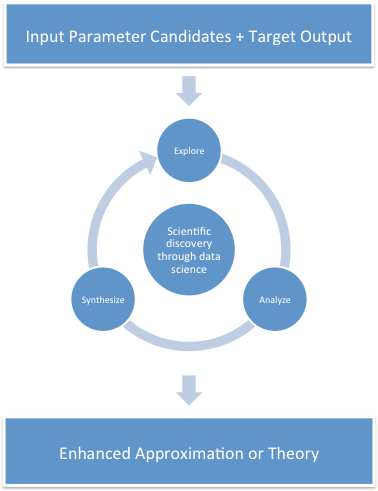
\includegraphics[width=.55\textwidth]{figs/chap1/dataCycle}
  \caption[Data Collection Cycle for Scientific Discovery]{A broad view of the exploratory data analysis pipeline under study.}
  \label{fig:dataCycle}
\end{figure}

\subsection{Experimentation}

In this body of work, we will be looking at experimental numeric data collected from various domains.
%
An experiment in our context is a procedure used to validate or invalidate some hypothesis set forth by the domain scientist.
%
The hypothesis usually seeks to define a relationship among different variable factors in a system under study.
%
A simulation is simply a computer experiment, i.e. a repeatable procedure with one or more variable input factors executed in a computational environment that produces one or more output factors to be analyzed.
%
Most of the applications in this work will be on simulations and not physical experiments, though from our standpoint, the difference is negligible as the methods described herein apply equally to both.
%
As such, we will use the term \textit{experiment} in order to be as general as possible.
%
In order to perform an experiment, we typically perform the procedure under different settings for a set of factors we believe to be significant.
%
Let us illustrate with an example.

In the scenario introduced above regarding nuclear fuel design, the first task for the scientist is quantify what denotes a ``safe'' fuel.
%
Next, the scientist will design one or more canonical scenarios by which to evaluate the safety of the fuel.
%
In designing these scenarios, the scientist is building a hypothesis about the factors that will affect the fuel's safety.
%
In the case where the factors can be quantified, the scientist will likely utilize some variation of the loop from Figure~\ref{fig:dataCycle}.
%
The scientist will thus generate and analyze data with the end goal of being able to further the mathematical understanding of nuclear fuel safety or to construct a reasonable approximation which can then be subjected to more extensive testing.

We specifically target multidimensional, numeric data which can be modeled as a scalar function.
%
A scalar function simply means that for a set of input parameters we associate a single target output value.
%
Multidimensional, in this setting, is taken to mean that the collection of inputs associated to the target value consists of two or more numeric values.
%
We will now take a moment to take a closer look at the specific problems to be addressed in each of the stages of the loop in Figure~\ref{fig:dataCycle}.

\subsection{Data Generation}

Due to the potentially large number of parameters that can be modified, an exhaustive search of the high-dimensional input space is rarely feasible.
%
To this end, researchers have developed both static and adaptive methods for intelligently sampling the input space.
%
Space-filling methods attempt to balance randomness with sampling density.
%
We review such space-filling techniques in Section~\ref{sec:forwardSampling}.

On the other hand, acknowledging that only a potentially small subspace of the input domain is interesting has led to the development of several adaptive algorithms that iteratively refine our understanding of the input space through careful selection of input samples.
%
The selection process is usually driven by an underyling model of the data that may favor areas of high uncertainty, steep gradient, low densitiy, or optimized values.
%
We review adaptive sampling techniques in Section~\ref{sec:adaptiveSampling}.
%
I present novel methods for injecting topology into the scoring and selection of candidates in the adaptive sampling process in Chapter~\ref{ch:adaptiveSampling}.

\subsection{Data Visualization}

In the initial stages of exploratory research, the scientist may have only a rudimentary understanding of the phenomenon of interest.
%
As such, s/he may formulate a broad hypothesis and begin by collecting large quantities of data for analysis without knowing what information is relevant at the time of collection.
%
Under such settings, we begin with a potentially sparse, sporadic, and noisy sampling of an input space with the hope of analyzing it with respect to some target value inherent in the data.
%
To effectively analze such data, s/he would first need to identify correlations and/or the lack thereof and eliminate extraneous dimensions or summarize collections of inputs into a reduced subspace of the problem.

To address these types of problems, researchers have developed a myriad of techniques ranging from the fully automated, such as dimensionality reduction and regression analysis, to highly user-driven exploratory analysis, like in the many visualization systems encoding sensitivity information.
%
These techniques are reviewed in Chapter~\ref{ch:related}.
%
In Section~\ref{paper:pacificVis2016}, I highlight novel, published work that explores the use of topological techniques for performing structured sensitivity analysis within a visualization system designed by the author for nuclear engineers.
%
This work is incorporated into the RAVEN software~\cite{RabitiAlfonsiCogliati2015} developed at Idaho National Laboratory and is currently used by nuclear engineers for analyzing experimental results ranging from nuclear fuel design to multi-plant coordination.

\subsection{Data Synthesis}

In the absence of developing a theoretical formula relating the inputs and outputs, we rely on approximations to represent the relationship between the target value and the inputs after analyzing the collected data.
%
We focus our attention on the construction of reduced order models (ROMs) through regression analysis and related techniques.
%
ROMs can be useful as an efficient and/or interpretable proxy for prediction or querying statistical or structural information about the acquired data.
%
ROMs range in their capacity to accurately fit data and also their interpretability creating a trade-off.
%
When selecting an appropriate ROM, there is no silver bullet, and one must consider the end goal before selecting an appropriate ROM.
%
I summarize the related efforts on regression analysis in Section~\ref{sec:regression}.

\bibliography{\jobname}